% ============================================================
%  Dispensa 01: Titoli obbligazionari — prezzo, rendimento,
%               duration e convexity
%  Corso di Calcolo Numerico — Laboratorio
%  Università degli Studi di Verona — A.A. 2026–2027
%  Prima lezione del corso: introduce, su un singolo titolo e un
%  singolo rendimento, gli stessi ingredienti numerici che le
%  dispense successive applicheranno a una curva intera —
%  ricerca di zeri e algebra lineare elementare (dispensa 02,
%  costruzione della curva RFR), troncamento ottimale e
%  combinazioni lineari (dispensa 03, PCA sui movimenti della
%  curva). Nessun dato esterno: i due titoli di esempio
%  sono definiti direttamente in R/01_bond_duration_convexity.R.
% ============================================================
\documentclass[11pt,a4paper]{article}

\usepackage[T1]{fontenc}
\usepackage[utf8]{inputenc}
\usepackage{textcomp}
\usepackage[italian]{babel}
\usepackage{lmodern}
\usepackage{amsmath,amssymb,amsthm,mathtools}
\usepackage{geometry}
\usepackage{booktabs}
\usepackage{array}
\usepackage{enumitem}
\usepackage{graphicx}
\usepackage{xcolor,colortbl}
\usepackage{hyperref}
\usepackage{float}
\usepackage{fancyvrb}
\usepackage{tcolorbox}
\tcbuselibrary{breakable}
\usepackage{titlesec}
\usepackage{bm}

% le figure sono prodotte da R/01_bond_duration_convexity.R in output/01_bond_duration_convexity/
\graphicspath{{../output/01_bond_duration_convexity/}}

\geometry{top=2.5cm,bottom=2.5cm,left=2.8cm,right=2.8cm}
\setlist[itemize]{topsep=4pt,itemsep=2pt,parsep=0pt}
\setlist[enumerate]{topsep=4pt,itemsep=2pt,parsep=0pt}
\hypersetup{colorlinks=true,linkcolor=blue!55!black,urlcolor=blue!55!black,
            citecolor=green!40!black}

\titleformat{\section}{\large\bfseries}{\thesection.}{0.55em}{}[{\vspace{1pt}\titlerule[0.4pt]}]
\titleformat{\subsection}{\normalsize\bfseries}{\thesubsection.}{0.55em}{}
\titleformat{\subsubsection}{\small\bfseries\itshape}{\thesubsubsection.}{0.5em}{}

% --- ambienti teorema ---
\theoremstyle{plain}
\newtheorem{teorema}{Teorema}[section]
\newtheorem{proposizione}[teorema]{Proposizione}
\theoremstyle{definition}
\newtheorem{definizione}[teorema]{Definizione}
\newtheorem{esempio}[teorema]{Esempio}
\theoremstyle{remark}
\newtheorem*{osservazione}{Osservazione}
\newtheorem*{attenzione}{Nota numerica}

% --- box colorati ---
\tcbset{
  mybase/.style={
    colback=gray!5, colframe=gray!40,
    boxrule=0.4pt, arc=2pt,
    left=7pt, right=7pt, top=5pt, bottom=5pt,
    fonttitle=\small\bfseries,
    breakable
  }
}
\newtcolorbox{keybox}[1][Concetto chiave]{mybase,
  colframe=blue!40!black, colback=blue!4, title={#1}}
\newtcolorbox{algobox}[1][Algoritmo]{mybase,
  colframe=teal!50!black, colback=teal!4, title={#1}}
\newtcolorbox{warningbox}{mybase,
  colframe=orange!70!black, colback=orange!5}
\newtcolorbox{codebox}[1][Codice R]{mybase,
  colframe=green!40!black, colback=green!3, title={#1}}

% --- colore righe tabella ---
\definecolor{rowtint}{RGB}{243,247,253}

% --- macro math ---
\newcommand{\R}{\mathbb{R}}
\newcommand{\N}{\mathbb{N}}
\newcommand{\YTM}{\mathrm{YTM}}
\newcommand{\abs}[1]{\left\lvert #1 \right\rvert}
\newcommand{\norm}[1]{\left\lVert #1 \right\rVert}
\newcommand{\defeq}{\coloneqq}

% ============================================================
\title{%
  \textbf{Titoli obbligazionari: prezzo, rendimento,\\ duration e convexity}\\[6pt]
  \large Dal singolo rendimento alla necessità di una curva dei tassi\\[4pt]
}
\author{Laboratorio di Calcolo Numerico --- Laurea Triennale in Matematica Applicata\\
  Universit\`a degli Studi di Verona\\[2pt]
  Anno Accademico 2026--2027}
\date{}

\begin{document}
\maketitle
\tableofcontents
\newpage

% ============================================================
\section{Motivazioni economiche}
% ============================================================

\subsection{Il problema: valutare oggi un flusso di pagamenti futuri}

Un'\textbf{obbligazione} (o \textbf{bond}) è un contratto con cui un emittente (uno Stato, una
banca, un'impresa) si impegna a pagare al possessore del titolo un flusso di importi prefissati
a date prefissate: le \textbf{cedole} periodiche più il rimborso del \textbf{nozionale} a
scadenza. È lo strumento finanziario più semplice e diffuso, ed è anche il punto di partenza
naturale per chiedersi: \emph{quanto vale oggi un pagamento che riceveremo in futuro?}

La risposta richiede due ingredienti: sapere \emph{quando} e \emph{quanto} si riceverà (i
flussi di cassa contrattuali, noti) e sapere \emph{a quale tasso} scontare quei flussi per
riportarli al presente (il \textbf{rendimento}, che invece va determinato). Il grosso di questa
dispensa consiste nel rendere precisi questi due concetti e nel risolvere, con strumenti di
calcolo numerico elementari, il problema \emph{inverso}: dato il prezzo a cui un titolo è
scambiato sul mercato, qual è il rendimento implicito?

\subsection{Obbligazioni, portafogli e gestione del rischio di tasso}

Chi possiede obbligazioni --- una banca, un fondo pensione, una compagnia di assicurazione ---
non è interessato soltanto al prezzo di oggi: vuole sapere \emph{quanto} quel prezzo si muove
se il rendimento di mercato cambia. Questa sensibilità ha un nome, \textbf{duration}, ed è la
prima e più importante misura di rischio di tasso di interesse: dice, in prima approssimazione,
di quanti punti percentuali varia il prezzo per un movimento di un punto percentuale del
rendimento. Una raffinatezza del second'ordine, la \textbf{convexity}, migliora questa stima
quando il movimento di tasso non è piccolo.

Queste due grandezze non sono un esercizio accademico: sono al centro della gestione
\textbf{attivo-passivo} (asset-liability management) delle compagnie assicurative e dei fondi
pensione, ed è esattamente per questa ragione --- rendere confrontabile il rischio di tasso di
attivi e passivi con scadenze diverse --- che il quadro regolamentare europeo Solvency~II
impone la costruzione di una curva dei tassi risk-free ufficiale, oggetto delle prossime
dispense.

\subsection{Il percorso di queste dispense}
\label{sec:percorso}

Questa lezione lavora con un \textbf{singolo titolo} e un \textbf{singolo rendimento} $y$: è la
situazione più semplice possibile, e permette di introdurre senza distrazioni gli strumenti
numerici --- ricerca di zeri, sviluppo di Taylor, algebra lineare elementare --- che il resto
del corso userà in contesti via via più ricchi. Il percorso ha tre tappe:
\begin{itemize}
  \item \textbf{01} (questa dispensa): \emph{un} titolo, \emph{un} rendimento $y$ costante per
        tutte le scadenze. Quanto vale il titolo, quanto rende, quanto si muove il suo prezzo
        se il rendimento cambia;
  \item \textbf{02}: il mercato quota rendimenti \emph{diversi} per scadenze diverse --- non
        basta più un numero, serve un'intera funzione $t\mapsto P(0,t)$. La \textbf{02}
        costruisce la curva risk-free ufficiale EIOPA con \emph{due} metodologie a confronto:
        il bootstrap (in vigore dal 2027) e Smith--Wilson (storica, 2016--2026);
  \item \textbf{03}: come si \emph{muove} nel tempo l'intera curva. Non più un solo $\Delta y$
        ma un vettore di variazioni, che l'analisi delle componenti principali (PCA)
        scompone in pochi movimenti elementari.
\end{itemize}

L'arco è quindi: \emph{un numero} $\to$ \emph{una curva} $\to$ \emph{i movimenti di una curva}.
La Sezione~\ref{sec:verso-curva} chiude la prima transizione, mostrando perché un singolo
rendimento non basta; la Sezione~\ref{sec:oltre-parallelo} chiude la seconda, mostrando perché
non basta nemmeno un singolo $\Delta y$.

\begin{osservazione}[Due curve diverse, lo stesso oggetto matematico]
Le due dispense successive non lavorano sulla stessa curva, ed è bene saperlo subito. La
\textbf{02} costruisce la curva \emph{regolamentare} EIOPA, ricavata da contratti swap e
imposta per legge a tutte le imprese assicurative europee; la \textbf{03} analizza la curva
\emph{di mercato} dei titoli di Stato dell'area euro con rating AAA, pubblicata dalla BCE.
Cambiano l'emittente, gli strumenti sottostanti e lo scopo --- ma l'oggetto matematico è
identico in entrambi i casi: una funzione che associa a ogni scadenza un fattore di sconto, e
tutto ciò che diremo su di essa vale per l'una come per l'altra.
\end{osservazione}

\paragraph{Gli strumenti numerici, e dove tornano.}
Per un corso di calcolo numerico conviene leggere il percorso anche in un secondo modo: non
per oggetti finanziari, ma per tecniche. Ognuna di quelle introdotte qui riappare più avanti,
sullo stesso schema ma su dati più grandi.

\begin{center}
\small
\renewcommand{\arraystretch}{1.35}
\begin{tabular}{@{}p{3.0cm} p{3.1cm} p{4.4cm} p{3.2cm}@{}}
\toprule
\textbf{Strumento} & \textbf{01} (questa) & \textbf{02} (curva RFR) & \textbf{03} (PCA)\\
\midrule
\rowcolor{rowtint}
Ricerca di zeri & $\YTM$: bisezione e Newton & forward nei gap (Newton); parametro $\alpha$ di
Smith--Wilson (bisezione) & ---\\
Sviluppo di Taylor & duration, convexity & --- & ---\\
\rowcolor{rowtint}
Sistemi lineari & immunizzazione $2\times2$ & triangolare per sostituzione in avanti
(bootstrap); denso e definito positivo (Smith--Wilson) & ---\\
Combinazioni lineari & duration di portafoglio & \textsc{llfr}: media pesata di forward &
\emph{scores} sui loadings\\
\rowcolor{rowtint}
Fattorizzazioni & --- & Cholesky & SVD\\
Troncamento ottimale & Taylor all'\textbf{ordine} $k$ & --- & SVD al \textbf{rango} $k$
(Eckart--Young)\\
\bottomrule
\end{tabular}
\end{center}

L'ultima riga merita un'osservazione, perché è il filo meno ovvio e il più istruttivo. In
questa dispensa tronchiamo uno sviluppo di Taylor al primo ordine (duration) o al secondo
(convexity), e misuriamo l'errore che resta (Sezione~\ref{sec:bonta}). Nella \textbf{03} si
tronca una decomposizione ai valori singolari, tenendo solo le prime $k$ componenti, e il
teorema di Eckart--Young garantisce che quel troncamento è il \emph{migliore possibile} a
parità di rango. Due volte la stessa idea --- tenere pochi termini e controllare quanto si
perde --- una volta nell'ordine di uno sviluppo, una volta nel rango di una matrice.

% ============================================================
\section{Prezzo e rendimento di un titolo obbligazionario}
% ============================================================

\subsection{Flussi di cassa di un titolo a cedola fissa}

Consideriamo un titolo con nozionale $N$, cedola annua $c$ (in percentuale del nozionale) e
scadenza $T$ anni, con pagamenti annuali. Il titolo genera i flussi di cassa
\[
  CF_t = \begin{cases} c\,N & t = 1,\ldots,T-1 \ \text{(sola cedola)},\\
                       c\,N + N & t = T \ \text{(cedola + rimborso del nozionale)}. \end{cases}
\]
Per semplicità consideriamo cedole \emph{annue}; il caso semestrale (o con altra frequenza) è
identico nella sostanza --- cambiano solo le date dei flussi --- ed è quello effettivamente
usato dal mercato IRS delle prossime dispense.

\subsection{Il prezzo come valore attuale}

\begin{definizione}[Prezzo di un'obbligazione]
\label{def:prezzo-bond}
Dato un rendimento $y > -1$ (lo stesso tasso per tutte le scadenze), il \textbf{prezzo} del
titolo è la somma dei valori attuali dei suoi flussi di cassa, scontati a capitalizzazione
annua composta:
\begin{equation}
  P(y) = \sum_{t=1}^{T} \frac{CF_t}{(1+y)^t}.
  \label{eq:prezzo}
\end{equation}
\end{definizione}

\subsection{Il caso elementare: lo zero-coupon bond}
\label{sec:zcb}

Il caso più semplice della Definizione~\ref{def:prezzo-bond} è quello di un titolo con un
\textbf{solo} flusso: nessuna cedola, solo il rimborso a scadenza. Merita un nome proprio
perché è il mattone con cui è costruito tutto il resto del corso.

\begin{definizione}[Zero-coupon bond e fattore di sconto]
\label{def:zcb}
Uno \textbf{zero-coupon bond} con scadenza $t$ paga un'unica unità di valuta al tempo $t$ e
nulla prima. Il suo prezzo di oggi si indica con $P(0,t)$ e si chiama \textbf{fattore di
sconto} per la scadenza $t$:
\begin{equation}
  P(0,t) = \frac{1}{(1+y_t)^{t}},
  \label{eq:zcb}
\end{equation}
dove $y_t$ è il rendimento associato a quella singola scadenza.
\end{definizione}

Con questa notazione la~\eqref{eq:prezzo} si riscrive come combinazione lineare di fattori di
sconto, $P = \sum_t CF_t\,P(0,t)$: prezzare un titolo qualsiasi significa conoscere i fattori
di sconto delle sue scadenze. In questa dispensa facciamo l'ipotesi drastica che sia
$y_t = y$ per ogni $t$ --- un solo rendimento per tutte le scadenze --- e infatti scriviamo
$P(y)$ e non $P(0,t)$. La \textbf{dispensa 02} rimuove esattamente questa ipotesi: il suo
oggetto è la funzione $t \mapsto P(0,t)$, e la \textbf{dispensa 03} studia come quella funzione
si muove nel tempo. Lo zero-coupon bond è dunque, letteralmente, l'unità di misura di entrambe.

\begin{keybox}[Le tre convenzioni di capitalizzazione]
Lo stesso fattore di sconto si scrive in modi diversi a seconda della convenzione, e le tre
dispense non usano tutte la stessa: conviene fissarle qui una volta per tutte.
\[
  \underbrace{P(0,t) = (1+y)^{-t}}_{\text{annua composta: questa dispensa}}
  \qquad
  \underbrace{P(0,t) = e^{-r^c t}}_{\text{continua: dispense 02 (interna) e 03}}
\]
Le due parametrizzazioni descrivono lo stesso prezzo e si convertono l'una nell'altra con
\begin{equation}
  1 + y = e^{r^c}, \qquad\text{cioè}\qquad r^c = \ln(1+y), \qquad y = e^{r^c}-1.
  \label{eq:conversione-capitalizzazione}
\end{equation}
La convenzione annua composta è quella con cui il mercato quota i titoli, ed è la ragione per
cui la usiamo qui; quella continua rende più pulite le formule di derivazione, ed è la ragione
per cui la curva EIOPA la usa internamente. Vedremo in
Sezione~\ref{sec:duration-modificata} che la scelta lascia una traccia visibile: il fattore
$1/(1+y)$ che distingue la duration modificata da quella di Macaulay sparisce in
capitalizzazione continua.
\end{keybox}

\subsection{Due titoli di esempio}
\label{sec:due-titoli}

Useremo, in tutta la dispensa, due titoli didattici (non quotazioni di mercato reali, nello
spirito degli esempi numerici di \cite{hull2018}, cap.~4):

\begin{center}
\renewcommand{\arraystretch}{1.3}
\begin{tabular}{lccc}
\toprule
Titolo & cedola $c$ & scadenza $T$ & prezzo di mercato $P_{\mathrm{mkt}}$ \\
\midrule
Bond A & 4\% & 5 anni & 97{,}50 \\
Bond B & 3\% & 10 anni & 96{,}00 \\
\bottomrule
\end{tabular}
\end{center}
Nozionale $N=100$ per entrambi. Entrambi quotano \emph{sotto la pari} ($P_{\mathrm{mkt}}<N$):
ci aspettiamo quindi, come vedremo tra poco, un rendimento superiore alla rispettiva cedola.

\subsection{Il rendimento a scadenza (YTM)}

Nella pratica la situazione è ribaltata rispetto alla Definizione~\ref{def:prezzo-bond}: il
mercato quota il \textbf{prezzo} $P_{\mathrm{mkt}}$, mentre il rendimento è \emph{incognito}.

\begin{definizione}[Rendimento a scadenza]
\label{def:ytm}
Il \textbf{rendimento a scadenza} (\emph{yield to maturity}, $\YTM$) di un titolo quotato al
prezzo $P_{\mathrm{mkt}}$ è il valore $y^\ast$ che risolve
\begin{equation}
  \varphi(y) \defeq P(y) - P_{\mathrm{mkt}} = 0.
  \label{eq:ytm-eq}
\end{equation}
\end{definizione}

La~\eqref{eq:ytm-eq} è un'equazione \emph{non lineare} in $y$: $P(y)$ è una somma di potenze
$(1+y)^{-t}$, non invertibile in forma chiusa per $T>1$. Serve un metodo numerico di ricerca
di zeri --- il tema della Sezione~\ref{sec:radici}.

\subsection{Monotonia e unicità del rendimento}

Prima di cercare $y^\ast$ conviene sapere che esiste ed è unico.

\begin{proposizione}[Monotonia del prezzo]
\label{prop:monotonia}
Per ogni titolo con flussi $CF_t>0$, la funzione $y\mapsto P(y)$ è strettamente decrescente su
$(-1,+\infty)$.
\end{proposizione}
La verifica è immediata derivando la~\eqref{eq:prezzo} termine a termine:
\begin{equation}
  P'(y) = -\sum_{t=1}^{T} \frac{t\,CF_t}{(1+y)^{t+1}} < 0 \qquad \text{per ogni } y>-1,
  \label{eq:dprezzo}
\end{equation}
essendo ogni addendo strettamente positivo (per $y>-1$ tutte le potenze $(1+y)^{t+1}$ sono
positive). Una funzione strettamente monotona è iniettiva: se una soluzione di
$\varphi(y)=0$ esiste, è \textbf{unica}. L'esistenza segue da $P(y)\to+\infty$ per
$y\to -1^+$ e $P(y)\to 0$ per $y\to+\infty$ (continuità + teorema degli zeri), purché
$0<P_{\mathrm{mkt}}$ sia un valore intermedio --- condizione sempre soddisfatta per un titolo
quotato a un prezzo positivo di mercato.

\begin{figure}[H]
\centering
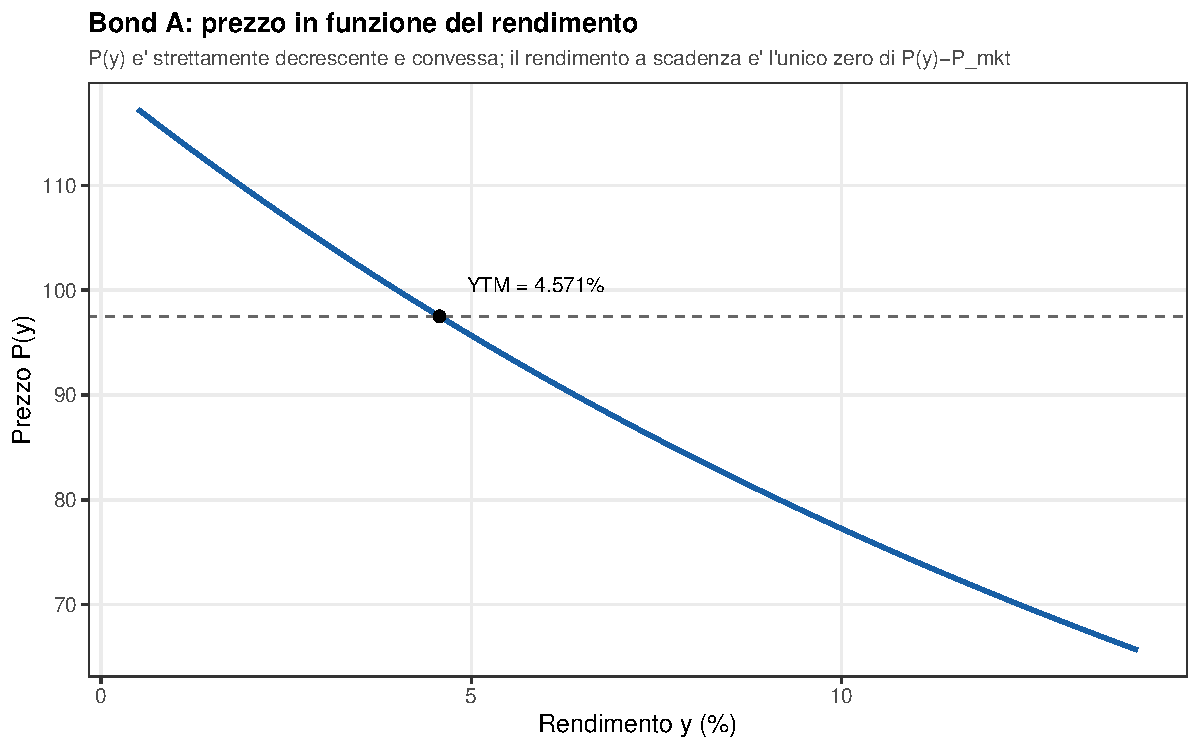
\includegraphics[width=0.85\textwidth]{fig_prezzo_rendimento.pdf}
\caption{Bond A: prezzo $P(y)$ in funzione del rendimento. La curva è strettamente decrescente
(Proposizione~\ref{prop:monotonia}) e convessa (Sezione~\ref{sec:convexity}): il rendimento a
scadenza è l'unico punto in cui la curva incrocia il prezzo di mercato (linea tratteggiata).}
\label{fig:prezzo-rendimento}
\end{figure}

% ============================================================
\section{Il calcolo del rendimento: bisezione e Newton-Raphson}
\label{sec:radici}
% ============================================================

\subsection{Il problema di ricerca di zeri}

La Proposizione~\ref{prop:monotonia} garantisce che $\varphi(y)=P(y)-P_{\mathrm{mkt}}$ ha
un'unica radice: resta da \textbf{calcolarla}. \`E il primo di una serie di problemi di ricerca
di zeri che attraverserà tutto il corso --- lo stesso schema tornerà, identico nella sostanza,
nella dispensa~02: per i tenor non consecutivi del bootstrap (risolti con Newton) e per la
calibrazione del parametro $\alpha$ di Smith--Wilson (risolta per bisezione). Qui lo
introduciamo nel caso più semplice: una sola equazione scalare, di cui conosciamo già segno e
monotonia.

\subsection{Bisezione}

Il metodo di \textbf{bisezione} sfrutta solo la continuità e il cambio di segno: se
$\varphi(a)$ e $\varphi(b)$ hanno segno opposto, il punto medio $m=(a+b)/2$ dimezza
l'intervallo che deve contenere lo zero, e si itera su $[a,m]$ o $[m,b]$ a seconda del segno di
$\varphi(m)$. La convergenza è \textbf{lineare}: l'ampiezza dell'intervallo si dimezza a ogni
passo, quindi servono $\approx \log_2((b-a)/\mathrm{tol})$ iterazioni per raggiungere una data
precisione --- lento ma infallibile, e per questo è lo standard di confronto ``robusto'' contro
cui misurare metodi più veloci (\cite{burden2016}, cap.~2; lo stesso ruolo che gioca nella
dispensa~02).

% GENERATO da R/01_bond_duration_convexity.R
\begin{table}[H]\centering\small
\caption{Bisezione su $[0,0.20]$ per il rendimento a scadenza del Bond A: punto medio $m_k$, residuo $\varphi(m_k)=P(m_k)-P_{\mathrm{mkt}}$ e ampiezza dell'intervallo. Si mostrano le prime 10 e le ultime 2 iterazioni.}
\label{tab:bisezione-ytm}\renewcommand{\arraystretch}{1.1}
\begin{tabular}{rccc}
\toprule
$k$ & $m_k$ (\%) & $\varphi(m_k)$ & ampiezza\\
\midrule
\rowcolor{rowtint}1 & 10.000000 & -2.024e+01 & 2.00e-01\\
2 & 5.000000 & -1.829e+00 & 1.00e-01\\
\rowcolor{rowtint}3 & 2.500000 & +9.469e+00 & 5.00e-02\\
4 & 3.750000 & +3.621e+00 & 2.50e-02\\
\rowcolor{rowtint}5 & 4.375000 & +8.480e-01 & 1.25e-02\\
6 & 4.687500 & -5.024e-01 & 6.25e-03\\
\rowcolor{rowtint}7 & 4.531250 & +1.699e-01 & 3.12e-03\\
8 & 4.609375 & -1.670e-01 & 1.56e-03\\
\rowcolor{rowtint}9 & 4.570312 & +1.239e-03 & 7.81e-04\\
10 & 4.589844 & -8.293e-02 & 3.91e-04\\
30 & 4.570600 & +5.398e-08 & 3.73e-10\\
$\vdots$ & $\vdots$ & $\vdots$ & $\vdots$\\
\rowcolor{rowtint}31 & 4.570600 & +1.382e-08 & 1.86e-10\\
\bottomrule
\end{tabular}
\end{table}


\subsection{Newton-Raphson}

Il metodo di \textbf{Newton-Raphson} sfrutta invece la derivata, disponibile qui in forma
chiusa dalla~\eqref{eq:dprezzo}: approssima $\varphi$ con la sua retta tangente e ne calcola lo
zero,
\begin{equation}
  y_{k+1} = y_k - \frac{\varphi(y_k)}{\varphi'(y_k)}, \qquad \varphi'(y) = P'(y).
  \label{eq:newton-ytm}
\end{equation}
Quando converge, lo fa \textbf{quadraticamente}: il numero di cifre corrette raddoppia a ogni
iterazione, a fronte del costo di calcolare anche la derivata. Una buona inizializzazione è
$y_0 = c$ (la cedola): il rendimento a scadenza tipicamente non se ne discosta troppo.

% GENERATO da R/01_bond_duration_convexity.R
\begin{table}[H]\centering\small
\caption{Newton-Raphson per il rendimento a scadenza del Bond A, inizializzato a $y_0=$ cedola $=4\%$. Il residuo crolla quadraticamente: gia' alla terza iterazione l'incremento e' sotto la precisione macchina.}
\label{tab:newton-ytm}\renewcommand{\arraystretch}{1.1}
\begin{tabular}{rccc}
\toprule
$k$ & $y_k$ (\%) & $\varphi(y_k)$ & $|y_k-y_{k-1}|$\\
\midrule
\rowcolor{rowtint}0 & 4.00000000 & +2.500e+00 & ---\\
1 & 4.56156778 & +3.895e-02 & 5.616e-03\\
\rowcolor{rowtint}2 & 4.57059766 & +9.823e-06 & 9.030e-05\\
3 & 4.57059994 & +6.537e-13 & 2.278e-08\\
\rowcolor{rowtint}4 & 4.57059994 & -2.842e-14 & 1.513e-15\\
\bottomrule
\end{tabular}
\end{table}


\subsection{Confronto numerico}

La Figura~\ref{fig:convergenza} confronta l'errore $\abs{y_k-y^\ast}$ dei due metodi sul Bond A,
in scala logaritmica: la bisezione scende con pendenza costante (convergenza lineare), Newton
precipita in poche iterazioni (convergenza quadratica) --- coerentemente con le
Tabelle~\ref{tab:bisezione-ytm} e~\ref{tab:newton-ytm}, dove Newton raggiunge la precisione di
macchina in 4 iterazioni contro le oltre 30 della bisezione.

\begin{figure}[H]
\centering
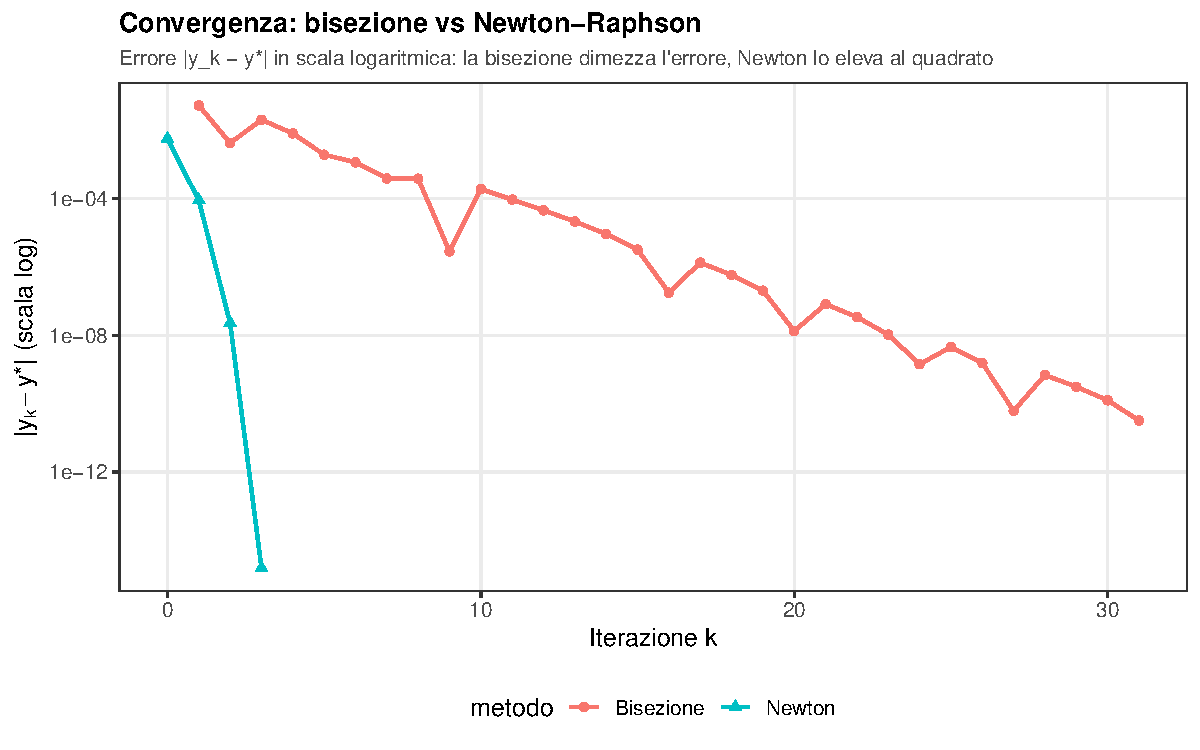
\includegraphics[width=0.85\textwidth]{fig_convergenza_bisezione_newton.pdf}
\caption{Bond A: errore $\abs{y_k-y^\ast}$ (scala log) per bisezione e Newton-Raphson. La
pendenza costante della bisezione è la firma della convergenza lineare; il crollo di Newton è
la firma della convergenza quadratica.}
\label{fig:convergenza}
\end{figure}

\begin{algobox}[Ricerca del rendimento a scadenza (in R)]
\begin{Verbatim}[fontsize=\small]
# cf, times: flussi di cassa e relative scadenze (anni)
bond_price  <- function(y, cf, times)  sum(cf / (1+y)^times)
bond_dprice <- function(y, cf, times) -sum(times * cf / (1+y)^(times+1))

phi  <- function(y) bond_price(y, cf, times) - Pmkt
dphi <- function(y) bond_dprice(y, cf, times)

# Newton-Raphson, inizializzato alla cedola
y <- c
repeat {
  y_new <- y - phi(y) / dphi(y)
  if (abs(y_new - y) < tol) break
  y <- y_new
}
\end{Verbatim}
\end{algobox}

% ============================================================
\section{Sensitivity: duration e convexity}
% ============================================================

\subsection{Lo sviluppo di Taylor del prezzo}

Trovato il rendimento a scadenza $y^\ast$ e il prezzo corrispondente $P_0=P(y^\ast)$, la
domanda successiva è: se il rendimento si sposta di una piccola quantità $\Delta y$, di quanto
si muove il prezzo? Rispondere ricalcolando $P(y^\ast+\Delta y)$ dalla~\eqref{eq:prezzo} è
sempre possibile, ma costoso se bisogna farlo per molti scenari o per molti titoli in
portafoglio. Lo \textbf{sviluppo di Taylor} di $P$ attorno a $y^\ast$ fornisce
un'approssimazione locale, in termini di sole due grandezze --- la derivata prima e la
derivata seconda in $y^\ast$ --- che si calcolano una volta sola:
\begin{equation}
  P(y^\ast+\Delta y) \;\approx\; P_0 + P'(y^\ast)\,\Delta y + \tfrac12 P''(y^\ast)\,\Delta y^2.
  \label{eq:taylor-P}
\end{equation}
Le prossime tre sottosezioni danno un nome finanziario a $P'(y^\ast)/P_0$ (duration modificata)
e a $P''(y^\ast)/P_0$ (convexity), riscrivendo la~\eqref{eq:taylor-P} in forma relativa.

\subsection{Duration di Macaulay}

\begin{definizione}[Duration di Macaulay]
\label{def:macaulay}
La \textbf{duration di Macaulay} è la media dei tempi di pagamento, pesata con il valore
attuale di ciascun flusso:
\begin{equation}
  D_{\mathrm{Mac}} = \sum_{t=1}^{T} t \cdot \frac{\mathrm{pv}_t}{P(y^\ast)},
  \qquad \mathrm{pv}_t \defeq \frac{CF_t}{(1+y^\ast)^t}.
  \label{eq:macaulay}
\end{equation}
\end{definizione}
Poiché i pesi $\mathrm{pv}_t/P$ sono positivi e sommano a 1, $D_{\mathrm{Mac}}$ è una media
pesata: un \textbf{baricentro temporale} dei flussi. Per un titolo con cedole $D_{\mathrm{Mac}}
< T$ sempre (parte del valore arriva prima della scadenza); per uno zero-coupon bond
$D_{\mathrm{Mac}}=T$ esattamente (un solo flusso, tutto il peso su di esso).

La Tabella~\ref{tab:flussi-bondA} mostra il calcolo completo per il Bond A: la colonna dei pesi
e quella del contributo $t\cdot$peso, la cui somma è $D_{\mathrm{Mac}}$.

% GENERATO da R/01_bond_duration_convexity.R
\begin{table}[H]\centering\small
\caption{Bond A: flussi di cassa, valore attuale al rendimento $y=4.5706\%$, peso $\mathrm{pv}_t/P$ e contributo $t\cdot\mathrm{pv}_t/P$ alla duration di Macaulay~\eqref{eq:macaulay}. La somma dell'ultima colonna \`e $D_{\mathrm{Mac}}$.}
\label{tab:flussi-bondA}\renewcommand{\arraystretch}{1.15}
\begin{tabular}{rcccc}
\toprule
$t$ (anni) & $CF_t$ & $\mathrm{pv}_t=CF_t(1+y)^{-t}$ & peso $\mathrm{pv}_t/P$ & $t\cdot$peso\\
\midrule
\rowcolor{rowtint}1 & 4.0000 & 3.8252 & 0.0392 & 0.0392\\
2 & 4.0000 & 3.6580 & 0.0375 & 0.0750\\
\rowcolor{rowtint}3 & 4.0000 & 3.4981 & 0.0359 & 0.1076\\
4 & 4.0000 & 3.3452 & 0.0343 & 0.1372\\
\rowcolor{rowtint}5 & 104.0000 & 83.1736 & 0.8531 & 4.2653\\
\midrule
\multicolumn{2}{r}{Somma (=$P$, =$D_{\mathrm{Mac}}$)} & 97.5000 & 1.0000 & 4.6245\\
\bottomrule
\end{tabular}
\end{table}


\subsection{Duration modificata}
\label{sec:duration-modificata}

\begin{definizione}[Duration modificata]
\label{def:modified}
La \textbf{duration modificata} è la derivata logaritmica del prezzo cambiata di segno,
\begin{equation}
  D_{\mathrm{mod}} \defeq -\frac{P'(y^\ast)}{P_0}.
  \label{eq:modified-def}
\end{equation}
\end{definizione}
Confrontando la~\eqref{eq:dprezzo} con la~\eqref{eq:macaulay} si trova la relazione, valida per
la capitalizzazione annua composta usata in questa dispensa,
\begin{equation}
  D_{\mathrm{mod}} = \frac{D_{\mathrm{Mac}}}{1+y^\ast}.
  \label{eq:mod-da-mac}
\end{equation}
Il fattore $1/(1+y^\ast)$ è il prezzo della convenzione discreta, come anticipato nel riquadro
di Sezione~\ref{sec:zcb}: se si lavorasse a capitalizzazione \emph{continua} (come fa
internamente la curva EIOPA nella dispensa~02) le due duration coinciderebbero esattamente,
perché $\frac{d}{dy}e^{-yt} = -t\,e^{-yt}$ senza alcun fattore correttivo.

Con $D_{\mathrm{mod}}$ la~\eqref{eq:taylor-P} tronca al 1\textsuperscript{o} ordine si scrive
in forma \textbf{relativa}, la forma in cui si trova quasi sempre nei testi:
\begin{equation}
  \frac{\Delta P}{P_0} \;\approx\; -D_{\mathrm{mod}}\,\Delta y.
  \label{eq:taylor-lineare}
\end{equation}
$D_{\mathrm{mod}}$ è dunque la \emph{sensibilità percentuale} del prezzo a un movimento di
tasso: un'obbligazione con $D_{\mathrm{mod}}=5$ perde circa il 5\% del suo valore per un rialzo
di 100 bps del rendimento.

\subsection{Convexity}
\label{sec:convexity}

\begin{definizione}[Convexity]
\label{def:convexity}
La \textbf{convexity} è il termine di secondo ordine, normalizzato allo stesso modo:
\begin{equation}
  C \defeq \frac{P''(y^\ast)}{P_0}
  = \frac{1}{P_0}\sum_{t=1}^{T} \frac{t(t+1)\,CF_t}{(1+y^\ast)^{t+2}} \;>\;0.
  \label{eq:convexity-def}
\end{equation}
\end{definizione}
$C>0$ sempre, per la stessa ragione della Proposizione~\ref{prop:monotonia}: ogni addendo è
positivo. Geometricamente è la curvatura di $P(y)$, già visibile in
Figura~\ref{fig:prezzo-rendimento}: la curva sta \emph{sopra} la propria retta tangente. Con la
convexity, la~\eqref{eq:taylor-P} tronca al 2\textsuperscript{o} ordine diventa
\begin{equation}
  \frac{\Delta P}{P_0} \;\approx\; -D_{\mathrm{mod}}\,\Delta y + \tfrac12\,C\,\Delta y^2.
  \label{eq:taylor-quadratica}
\end{equation}
Il segno $+$ davanti a $C$ è una buona notizia per chi detiene il titolo: la convexity
\emph{attenua} le perdite quando i tassi salgono e \emph{amplifica} i guadagni quando i tassi
scendono, un'asimmetria a favore dell'obbligazionista.

La Tabella~\ref{tab:riepilogo-duration} riassume $\YTM$, $D_{\mathrm{Mac}}$, $D_{\mathrm{mod}}$
e $C$ per entrambi i titoli di esempio: il Bond B, con scadenza doppia, ha duration e
convexity molto più alte --- è più sensibile ai movimenti di tasso, come ci si aspetta da un
titolo più lungo.

% GENERATO da R/01_bond_duration_convexity.R
\begin{table}[H]\centering\small
\caption{Riepilogo dei due titoli di esempio al proprio rendimento a scadenza.}
\label{tab:riepilogo-duration}\renewcommand{\arraystretch}{1.15}
\begin{tabular}{lccccccc}
\toprule
Titolo & cedola & $T$ & $P_{\mathrm{mkt}}$ & YTM (\%) & $D_{\mathrm{Mac}}$ & $D_{\mathrm{mod}}$ & $C$\\
\midrule
\rowcolor{rowtint}Bond A & 4\% & 5 & 97.50 & 4.5706 & 4.6245 & 4.4223 & 24.7025\\
Bond B & 3\% & 10 & 96.00 & 3.4805 & 8.7560 & 8.4615 & 85.8768\\
\bottomrule
\end{tabular}
\end{table}


\subsection{Bontà dell'approssimazione}
\label{sec:bonta}

Quanto sono buone le approssimazioni~\eqref{eq:taylor-lineare}
e~\eqref{eq:taylor-quadratica}? La Figura~\ref{fig:taylor-prezzo} sovrappone il prezzo esatto
del Bond A alle due approssimazioni al variare di $\Delta y$; la
Figura~\ref{fig:taylor-errore} e la Tabella~\ref{tab:taylor-confronto} quantificano l'errore in
punti base di prezzo.

\begin{figure}[H]
\centering
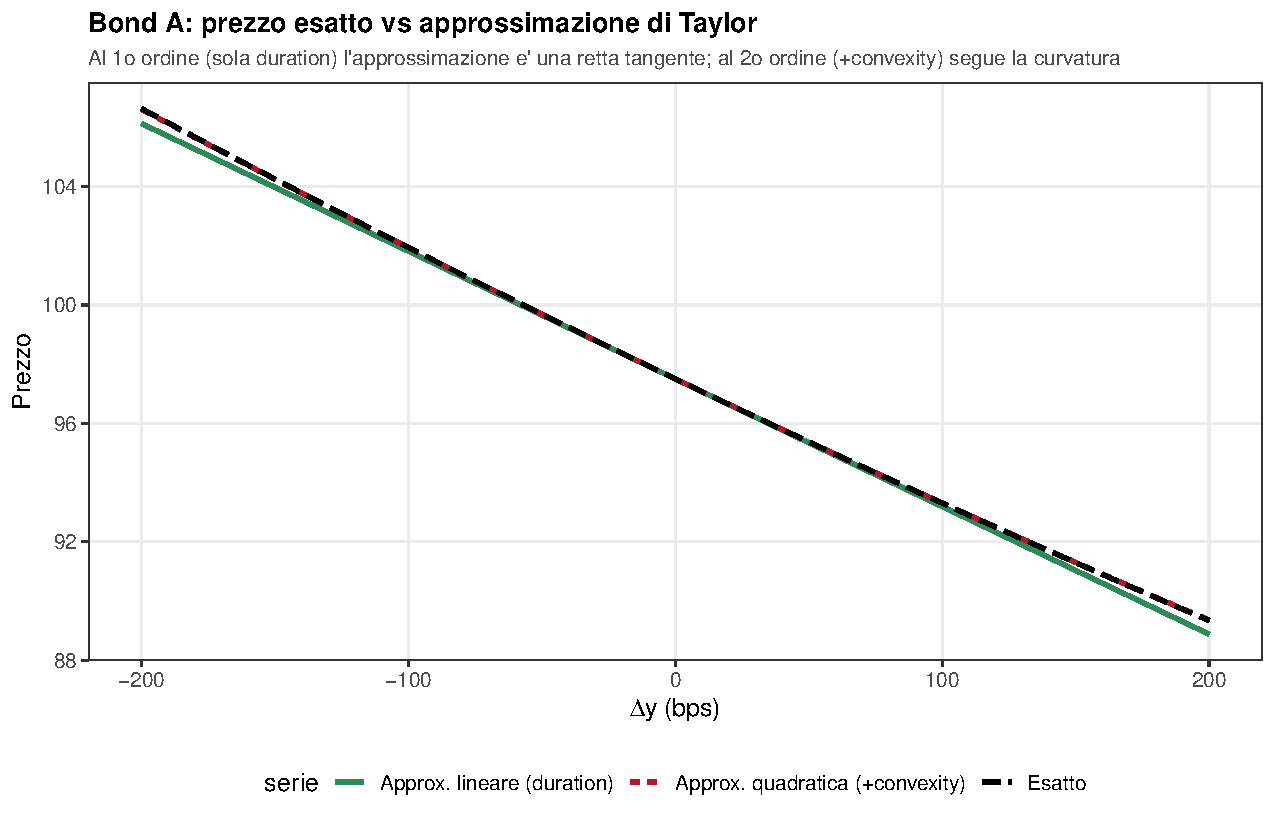
\includegraphics[width=0.88\textwidth]{fig_taylor_prezzo.pdf}
\caption{Bond A: prezzo esatto vs approssimazioni di Taylor al 1\textsuperscript{o} e
2\textsuperscript{o} ordine. Per $\Delta y$ piccoli le tre curve sono indistinguibili; per
$\Delta y$ grandi la sola duration (retta tangente) si allontana visibilmente dall'esatto,
mentre la correzione di convexity la insegue.}
\label{fig:taylor-prezzo}
\end{figure}

\begin{figure}[H]
\centering
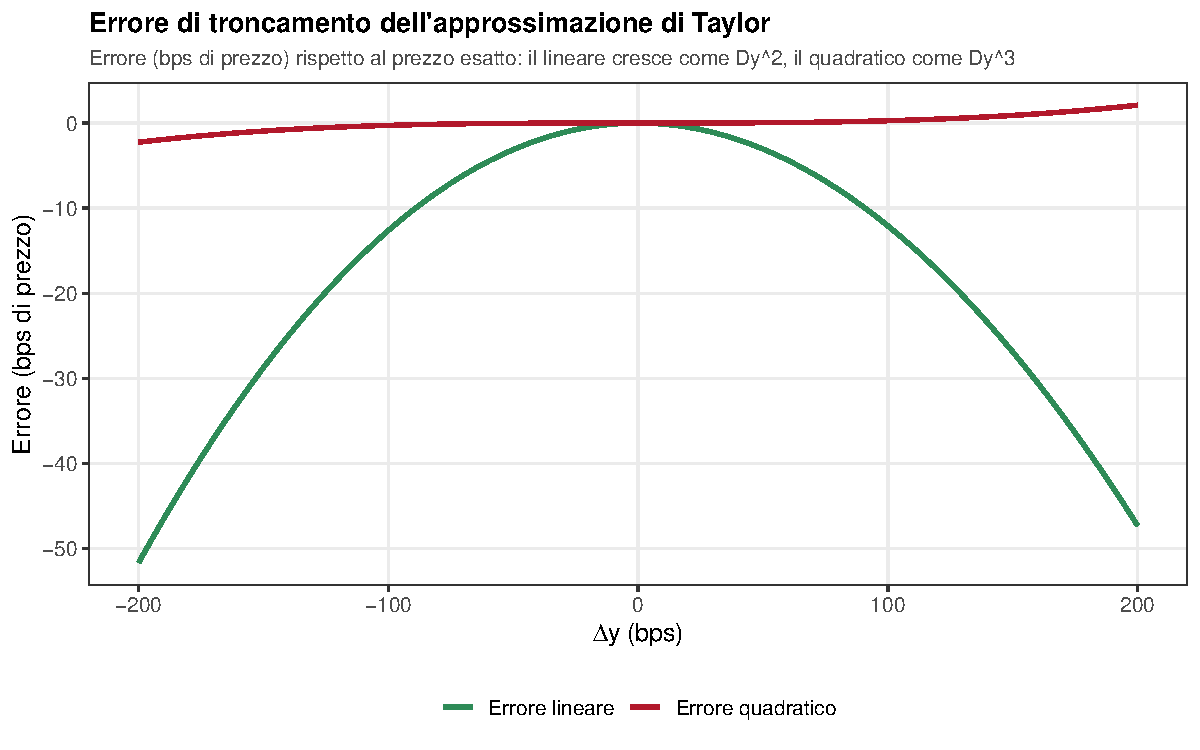
\includegraphics[width=0.85\textwidth]{fig_taylor_errore.pdf}
\caption{Bond A: errore di troncamento (bps di prezzo) delle due approssimazioni. L'errore
lineare cresce come $\Delta y^2$ (resta il termine di convexity trascurato), quello quadratico
come $\Delta y^3$ --- una cifra di precisione in più per ogni raddoppio della finezza dello
sviluppo.}
\label{fig:taylor-errore}
\end{figure}

% GENERATO da R/01_bond_duration_convexity.R
\begin{table}[H]\centering\small
\caption{Bond A: prezzo esatto e approssimazioni di Taylor al 1\textsuperscript{o} e 2\textsuperscript{o} ordine, per diversi shock $\Delta y$. Errore in bps di prezzo rispetto all'esatto.}
\label{tab:taylor-confronto}\renewcommand{\arraystretch}{1.15}
\begin{tabular}{rccccc}
\toprule
$\Delta y$ (bps) & esatto & lineare & quadratico & err. lineare (bps) & err. quadr. (bps)\\
\midrule
\rowcolor{rowtint}-200 & 106.6273 & 106.1235 & 106.6052 & -51.67 & -2.261\\
-100 & 101.9349 & 101.8118 & 101.9322 & -12.63 & -0.277\\
\rowcolor{rowtint}-50 & 99.6863 & 99.6559 & 99.6860 & -3.12 & -0.034\\
-25 & 98.5855 & 98.5779 & 98.5855 & -0.78 & -0.004\\
\rowcolor{rowtint}+0 & 97.5000 & 97.5000 & 97.5000 & +0.00 & +0.000\\
+25 & 96.4295 & 96.4221 & 96.4296 & -0.77 & +0.004\\
\rowcolor{rowtint}+50 & 95.3739 & 95.3441 & 95.3742 & -3.05 & +0.034\\
+100 & 93.3061 & 93.1882 & 93.3087 & -12.08 & +0.267\\
\rowcolor{rowtint}+200 & 89.3377 & 88.8765 & 89.3582 & -47.31 & +2.095\\
\bottomrule
\end{tabular}
\end{table}


\begin{osservazione}[Errore di troncamento, non di arrotondamento]
Gli errori di Tabella~\ref{tab:taylor-confronto} non hanno nulla a che fare con la precisione
di macchina: sono l'errore di troncamento intrinseco dello sviluppo di Taylor, esattamente
analogo a quello studiato per l'interpolazione polinomiale. Raddoppiando $\Delta y$ l'errore
lineare quadruplica e quello quadratico ottuplica --- si legga la Tabella~\ref{tab:taylor-confronto}
confrontando le righe a $\pm 50$ e $\pm 100$ bps.
\end{osservazione}

% ============================================================
\section{Duration di portafoglio e immunizzazione}
% ============================================================

\subsection{Duration di portafoglio}

Chi detiene più titoli è interessato alla sensibilità dell'intero portafoglio, non dei singoli
titoli. Se un portafoglio di valore totale $V$ è composto da titoli di valore $V_i$ (pesi
$w_i=V_i/V$, $\sum_i w_i=1$) e duration modificata $D_i$, la duration del portafoglio è
semplicemente la \textbf{media pesata}
\begin{equation}
  D_{\mathrm{port}} = \sum_i w_i\, D_i,
  \label{eq:duration-portafoglio}
\end{equation}
perché il prezzo del portafoglio è la somma dei prezzi, e la derivata di una somma è la somma
delle derivate. \`E il primo uso, in questo corso, di una combinazione lineare per aggregare
grandezze finanziarie di titoli diversi --- lo stesso principio, in forma via via più elaborata,
tornerà nella media pesata dei forward della dispensa~02 e nella proiezione su
componenti principali della dispensa~03.

\subsection{Immunizzazione}

Un fondo pensione o una compagnia assicurativa hanno passività (pagamenti futuri dovuti agli
assicurati) oltre che attività (il portafoglio obbligazionario che le finanzia). Se attivo e
passivo hanno duration diverse, un movimento dei tassi li fa muovere in modo diverso e crea uno
squilibrio patrimoniale. L'\textbf{immunizzazione} elementare consiste nello scegliere i pesi
del portafoglio in modo che la sua duration coincida con quella della passività da coprire:
dati due titoli con duration modificata $D_A\neq D_B$ e una passività di duration modificata
target $D_L$, si risolve il sistema lineare $2\times 2$
\begin{equation}
  \begin{cases} w_A + w_B = 1\\[2pt] w_A D_A + w_B D_B = D_L \end{cases}
  \quad\Longrightarrow\quad
  w_A = \dfrac{D_L - D_B}{D_A - D_B}, \qquad w_B = 1-w_A.
  \label{eq:immunizzazione}
\end{equation}
\`E esattamente questo tipo di vincolo --- rendere il rischio di tasso di attivo e passivo
confrontabile --- a motivare, in Solvency~II, l'uso di un'unica curva dei tassi ufficiale
per tutte le imprese (Sezione~\ref{sec:verso-curva}).

\subsection{Esempio numerico}

Immunizziamo una passività unica --- un solo pagamento futuro, cioè uno zero-coupon bond nel
senso della Definizione~\ref{def:zcb} --- con scadenza $T_L=7$ anni, usando un portafoglio
composto dai due titoli di Sezione~\ref{sec:due-titoli}.

Restano due dettagli da fissare, entrambi istruttivi. Il primo: la passività scade a 7 anni,
ma i titoli disponibili scadono a 5 e a 10. Che rendimento attribuirle? Non avendo (ancora)
una curva, la ricaviamo per \textbf{interpolazione lineare} fra $y_A$ e $y_B$, ottenendo
$y_L \approx 4{,}13\%$. È una scorciatoia, e il fatto stesso di doverla prendere è un primo
sintomo del limite di questa lezione: ricostruire i rendimenti alle scadenze non quotate è
precisamente il problema che la dispensa~02 affronta sul serio.

Il secondo: quale duration allineare. La grandezza che governa il P\&L è la duration
\textbf{modificata} --- è lei a comparire nella~\eqref{eq:taylor-lineare} --- e su quella
imponiamo l'uguaglianza. Non è un cavillo: essendo $D_{\mathrm{mod}}=D_{\mathrm{Mac}}/(1+y)$ e
avendo i due titoli rendimenti \emph{diversi} ($4{,}57\%$ e $3{,}48\%$), allineare le Macaulay
lascerebbe le modificate disallineate, e il portafoglio non sarebbe immunizzato nemmeno contro
lo spostamento parallelo.

La Figura~\ref{fig:immunizzazione} mostra la duration modificata del portafoglio al variare del
peso $w_A$: una retta (per la linearità della~\eqref{eq:duration-portafoglio}) che incrocia il
target $D_{\mathrm{mod}}^{L}=T_L/(1+y_L)$ in un unico punto, i cui pesi sono riportati in
Tabella~\ref{tab:immunizzazione}.

\begin{figure}[H]
\centering
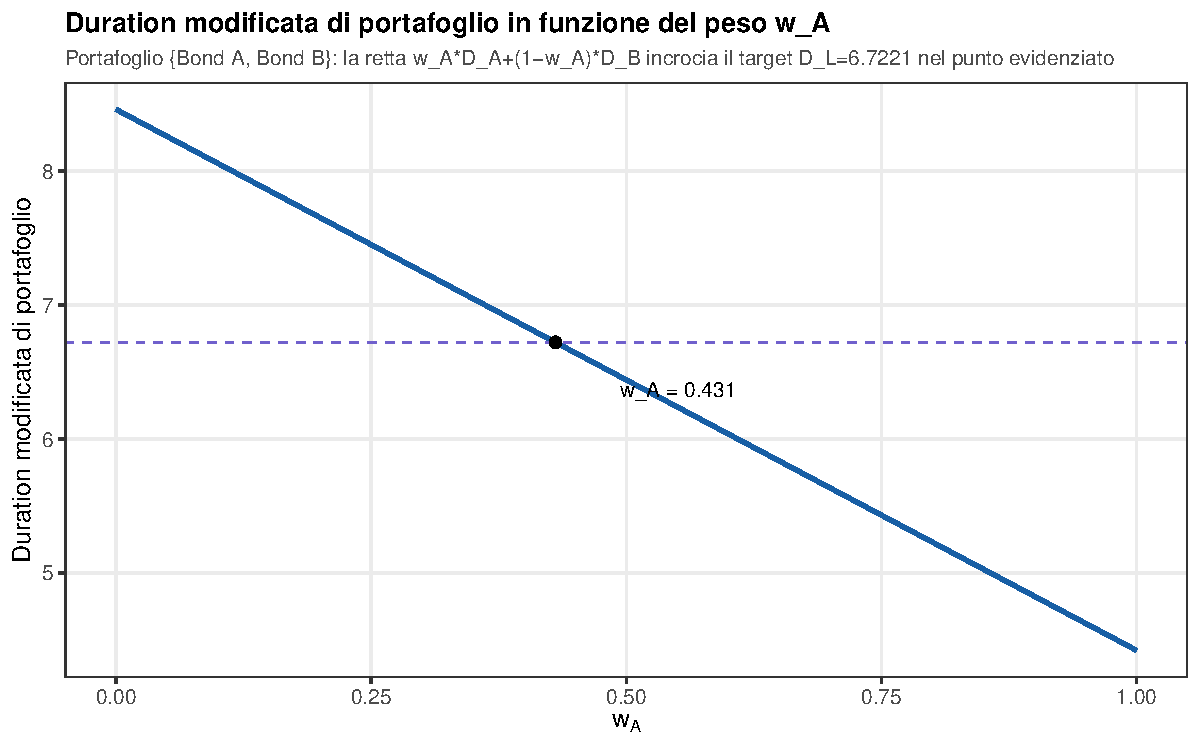
\includegraphics[width=0.85\textwidth]{fig_immunizzazione.pdf}
\caption{Duration modificata del portafoglio $\{$Bond A, Bond B$\}$ in funzione del peso $w_A$
(eq.~\eqref{eq:duration-portafoglio}). Il punto evidenziato è la soluzione
della~\eqref{eq:immunizzazione} per la passività zero-coupon a $T_L=7$ anni.}
\label{fig:immunizzazione}
\end{figure}

% GENERATO da R/01_bond_duration_convexity.R
\begin{table}[H]\centering\small
\caption{Immunizzazione di una passivit\`a zero-coupon a $T_L=7$ anni con il portafoglio $\{$Bond A, Bond B$\}$: pesi che risolvono il sistema~\eqref{eq:immunizzazione} e grandezze risultanti. Si allineano le duration \emph{modificate}, che sono quelle che governano il P\&L.}
\label{tab:immunizzazione}\renewcommand{\arraystretch}{1.15}
\begin{tabular}{lc}
\toprule
\rowcolor{rowtint}rendimento della passivit\`a $y_L$ (interpolato, \%) & 4.1346\\
target $D_{\mathrm{mod}}^{L} = T_L/(1+y_L)$ & 6.7221\\
\rowcolor{rowtint}peso Bond A, $w_A$ & 0.4306\\
peso Bond B, $w_B=1-w_A$ & 0.5694\\
\rowcolor{rowtint}duration modificata di portafoglio & 6.7221\\
convexity di portafoglio $C_{\mathrm{port}}$ & 59.5324\\
\rowcolor{rowtint}convexity della passivit\`a $C_L$ & 51.6414\\
\bottomrule
\end{tabular}
\end{table}


\begin{osservazione}
L'immunizzazione per matching di duration protegge solo da spostamenti \emph{paralleli e
piccoli} della curva dei tassi (coerentemente con l'approssimazione lineare
della~\eqref{eq:taylor-lineare}, qui applicata titolo per titolo). Le due restrizioni non sono
equivalenti, e conviene tenerle distinte: quella su ``piccoli'' è un limite di \emph{ordine},
già misurato in Sezione~\ref{sec:bonta} e correggibile con la convexity; quella su
``paralleli'' è un limite di \emph{forma}, e non si corregge affinando lo sviluppo di Taylor.
La Sezione~\ref{sec:oltre-parallelo} la mette alla prova con un esperimento numerico.
\end{osservazione}

% ============================================================
\section{Dal rendimento singolo alla curva dei tassi}
\label{sec:verso-curva}
% ============================================================

Il modello di questa dispensa ha un limite strutturale, visibile già nei due titoli di
esempio: il Bond A (5 anni) e il Bond B (10 anni) hanno rendimenti a scadenza \emph{diversi}
(rispettivamente $\approx 4{,}57\%$ e $\approx 3{,}48\%$, Tabella~\ref{tab:riepilogo-duration}),
pur essendo entrambi titoli di alta qualità nella stessa valuta. Non esiste, nella realtà, ``il''
rendimento di mercato: esiste un rendimento diverso per ogni scadenza. L'insieme di questi
rendimenti al variare della scadenza è la \textbf{struttura a termine dei tassi di interesse},
o curva dei tassi.

\begin{keybox}[Perché serve una curva, non un numero]
Un unico $y$ può prezzare correttamente \emph{un} titolo (per costruzione, è il suo YTM), ma
non è in generale coerente con il prezzo di un secondo titolo a scadenza diversa: usare lo YTM
del Bond A per scontare i flussi del Bond B darebbe un prezzo sbagliato. Per prezzare
\emph{simultaneamente} titoli di scadenze diverse in modo coerente (nessun arbitraggio) serve
una funzione $t\mapsto P(0,t)$ --- un fattore di sconto per ogni scadenza, non un rendimento
unico per tutte.
\end{keybox}

Costruire questa funzione a partire dai prezzi di mercato --- che tipicamente non coprono ogni
scadenza possibile, esattamente come qui avevamo solo due titoli a 5 e 10 anni, e come si è
visto interpolando a mano il rendimento a 7 anni della passività --- è il problema di cui si
occupa la \textbf{dispensa~02}, che lo risolve con due metodologie messe a confronto: il
bootstrap e Smith--Wilson. Il vocabolario che introdurrà --- fattore di sconto, tasso spot,
tasso forward --- è la naturale generalizzazione del rendimento $y$ di questa lezione al caso
di una curva intera.

% ============================================================
\section{Quando lo spostamento parallelo non basta}
\label{sec:oltre-parallelo}
% ============================================================

C'è un secondo limite, indipendente dal primo, e si vede meglio \emph{dopo} aver ammesso che
esiste una curva. Fin qui la domanda ``di quanto si muove il prezzo se i tassi cambiano'' aveva
una risposta governata da un solo numero, $\Delta y$. Ma se a ogni scadenza corrisponde un
rendimento diverso, allora anche il \emph{movimento} ha una scadenza per componente: non un
numero ma un vettore
\[
  \Delta r = \bigl(\Delta r(T_1),\, \Delta r(T_2),\, \ldots,\, \Delta r(T_n)\bigr) \in \R^n .
\]
La duration risponde alla domanda solo nel caso particolare in cui tutte le componenti di
$\Delta r$ sono \emph{uguali fra loro} --- il cosiddetto \textbf{spostamento parallelo}. Non è
un'ipotesi innocua, ed è facile verificarlo.

\subsection{Un esperimento: la stessa ampiezza, tre forme diverse}

Prendiamo il portafoglio appena immunizzato e sottoponiamolo a tre movimenti di tassi, tutti
della stessa ampiezza ($25$ bps), ma di \emph{forma} diversa. Poiché qui la ``curva'' consiste
di soli tre punti --- le scadenze $5$, $7$ e $10$ anni, cioè i due titoli e la passività ---
bastano tre numeri per descrivere ciascuno scenario (Figura~\ref{fig:shock-non-paralleli}):
\begin{itemize}
  \item \textbf{parallelo}: tutte e tre le scadenze salgono di $25$ bps;
  \item \textbf{irripidimento}: la scadenza breve scende di $25$ bps, la lunga sale di $25$
        bps, il punto a 7 anni resta fermo --- la curva ruota, diventando più inclinata;
  \item \textbf{appiattimento}: la rotazione opposta.
\end{itemize}
Nessuno dei tre è più ``grande'' degli altri: cambia solo come l'ampiezza è distribuita fra le
scadenze.

\begin{figure}[H]
\centering
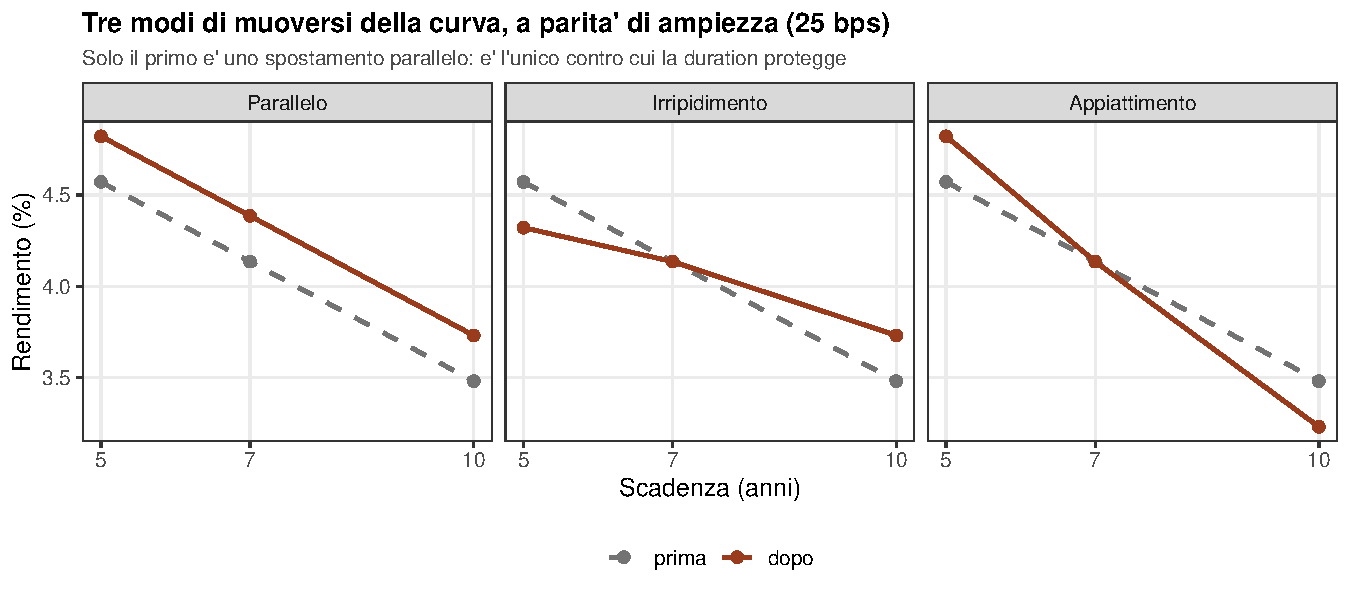
\includegraphics[width=0.95\textwidth]{fig_shock_non_paralleli.pdf}
\caption{I tre scenari sui tre nodi rilevanti ($5$, $7$ e $10$ anni). Tratteggiata la
situazione di partenza, continua quella dopo lo shock. L'ampiezza dello spostamento è la stessa
in tutti e tre i casi: cambia solo la forma.}
\label{fig:shock-non-paralleli}
\end{figure}

I prezzi vengono ricalcolati in modo \textbf{esatto} con la~\eqref{eq:prezzo}, non con
l'approssimazione di duration: quello che si misura è il vero profitto e perdita, non la sua
stima lineare.

% GENERATO da R/01_bond_duration_convexity.R
\begin{table}[H]\centering\small
\caption{Il portafoglio immunizzato della Tabella~\ref{tab:immunizzazione} sottoposto a tre movimenti di ampiezza identica ($25$~bps), con prezzi ricalcolati in modo \emph{esatto} su una base di 100. Lo shift parallelo lascia il netto praticamente nullo (resta solo il divario di convexity); le due rotazioni no, pur muovendo i tassi della stessa quantit\`a.}
\label{tab:shock-immunizzazione}\renewcommand{\arraystretch}{1.25}
\begin{tabular}{lcccrrr}
\toprule
\textbf{Scenario} & \multicolumn{3}{c}{shock (bps)} & $\Delta$ attivo & $\Delta$ passivo & \textbf{netto}\\
\cmidrule(lr){2-4}\cmidrule(lr){5-7}
& 5 anni & 7 anni & 10 anni & & & \\
\midrule
\rowcolor{rowtint}Parallelo & +25 & +25 & +25 & -1.6621 & -1.6645 & \textbf{+0.0024}\\
Irripidimento & -25 & 0 & +25 & -0.7098 & +0.0000 & \textbf{-0.7098}\\
\rowcolor{rowtint}Appiattimento & +25 & 0 & -25 & +0.7470 & +0.0000 & \textbf{+0.7470}\\
\bottomrule
\end{tabular}
\end{table}


Il risultato è netto. Nello scenario parallelo attivo e passivo perdono quasi esattamente lo
stesso importo ($-1{,}66$ su una base di $100$) e il saldo resta a $+0{,}0024$: il portafoglio
è immunizzato, come promesso. Nei due scenari di rotazione il passivo non si muove affatto ---
il suo unico flusso sta a 7 anni, e il punto a 7 anni è il perno della rotazione --- mentre
l'attivo sì, e il saldo salta a $-0{,}71$ e $+0{,}75$ rispettivamente: quasi \emph{trecento
volte} il residuo del caso parallelo.

\begin{keybox}[Che cosa ha fallito, esattamente]
Non è un errore di calcolo né un problema di ordine di approssimazione: aggiungere la convexity
non sistemerebbe nulla, perché lo scarto non nasce dall'ampiezza del movimento ma dalla sua
\emph{forma}. Imponendo una sola uguaglianza (quella fra le duration modificate) abbiamo
protetto il portafoglio lungo \emph{una sola direzione} nello spazio dei movimenti possibili.
Il vettore $\Delta r$ vive in $\R^n$; la duration ne controlla una dimensione sola.
\end{keybox}

\subsection{Quante direzioni servono davvero}

La domanda diventa allora: quante e quali direzioni contano? Se ne servissero $n$ (una per
scadenza) il problema sarebbe intrattabile. Il fatto notevole --- osservato per la prima volta
da Litterman e Scheinkman~\cite{litterman1991} e verificato su tutti i mercati obbligazionari
da allora --- è che ne bastano pochissime, e che hanno una forma riconoscibile e stabile:
\begin{itemize}
  \item \textbf{livello}: tutte le scadenze si muovono insieme, nella stessa direzione. È
        esattamente lo spostamento parallelo di cui sopra --- l'unico che la duration cattura;
  \item \textbf{pendenza}: brevi e lunghe si muovono in direzioni opposte. Sono i due scenari
        di rotazione che hanno fatto fallire l'immunizzazione;
  \item \textbf{curvatura}: il centro della curva si muove in senso opposto ai due estremi.
\end{itemize}
Sulla curva dei tassi dell'area euro degli ultimi vent'anni questi tre movimenti spiegano
rispettivamente circa l'$89{,}7\%$, l'$8{,}4\%$ e l'$1{,}4\%$ della variabilità osservata: il
$99{,}5\%$ del totale con tre soli numeri al posto di venti.

La duration copre dunque il primo --- di gran lunga il più importante, ed è la ragione per cui
è comunque la prima misura di rischio che si guarda --- e ignora gli altri due, che insieme
valgono circa il $10\%$ dei movimenti. Il portafoglio della Tabella~\ref{tab:immunizzazione}
è protetto contro il $90\%$ di ciò che può accadere, e scoperto sul restante $10\%$: quanto
basta, come si è visto, per perdere $0{,}71$ su $100$ in uno scenario tutt'altro che estremo.

Come si trovino quelle tre direzioni --- e come si dimostri che sono le \emph{migliori} tre
possibili, non semplicemente tre ragionevoli --- è l'oggetto della \textbf{dispensa~03}: la
risposta passa dalla decomposizione ai valori singolari e dal teorema di Eckart--Young, cioè
dallo stesso principio di troncamento ottimale già incontrato qui con lo sviluppo di Taylor.

% ============================================================
\section{Conclusioni}
% ============================================================

\begin{itemize}
  \item Il \textbf{prezzo} di un'obbligazione è il valore attuale dei suoi flussi di cassa a un
        rendimento $y$; il caso elementare con un solo flusso definisce il \textbf{fattore di
        sconto} $P(0,t)$, l'unità di misura di tutto il corso. Il \textbf{rendimento a
        scadenza} è il valore di $y$ che riprezza esattamente il titolo quotato sul mercato ---
        un problema di \textbf{ricerca di zeri} (bisezione, robusta ma lineare; Newton-Raphson,
        quadratico ma bisognoso della derivata), risolto qui per la prima volta e ritrovato,
        nella stessa forma, nella dispensa~02.
  \item La \textbf{duration di Macaulay} è il baricentro temporale dei flussi; la
        \textbf{duration modificata} e la \textbf{convexity} sono il 1\textsuperscript{o} e il
        2\textsuperscript{o} termine dello sviluppo di \textbf{Taylor} del prezzo rispetto al
        rendimento, e quantificano quanto bene un'approssimazione lineare (o quadratica)
        sostituisce un ricalcolo esatto.
  \item La \textbf{duration di portafoglio} è una media pesata delle duration dei singoli
        titoli --- prima comparsa, in questo corso, di una combinazione lineare elementare per
        aggregare grandezze finanziarie --- e sta alla base dell'\textbf{immunizzazione} di una
        passività, la motivazione pratica per cui la gestione del rischio di tasso richiede una
        curva dei tassi comune e condivisa.
  \item Il modello di questa lezione ha \textbf{due limiti}, che aprono le due dispense
        successive. Un singolo rendimento $y$ non descrive titoli di scadenze diverse: serve
        una \textbf{curva} $t\mapsto P(0,t)$, ed è la dispensa~02 a costruirla (bootstrap e
        Smith--Wilson a confronto). E una singola duration non descrive tutti i modi in cui
        quella curva può muoversi: serve \textbf{decomporne i movimenti}, ed è la dispensa~03 a
        farlo (PCA e SVD). L'esperimento della Sezione~\ref{sec:oltre-parallelo} mostra
        quantitativamente il secondo limite: un portafoglio immunizzato regge lo spostamento
        parallelo e cede a una rotazione della stessa ampiezza.
\end{itemize}

% ============================================================
\renewcommand{\refname}{Riferimenti bibliografici}
\begin{thebibliography}{9}

\bibitem{hull2018}
  \textbf{Hull, J.C.} (2018).
  \textit{Options, Futures, and Other Derivatives}, 10th ed. Pearson.
  Cap.~4: valore temporale del denaro, tassi di interesse, prezzo e rendimento delle
  obbligazioni, duration e convexity.

\bibitem{fabozzi2012}
  \textbf{Fabozzi, F.J.} (2012).
  \textit{Bond Markets, Analysis, and Strategies}, 8th ed. Pearson.
  Riferimento classico su duration, convexity e immunizzazione di portafoglio.

\bibitem{litterman1991}
  \textbf{Litterman, R., Scheinkman, J.} (1991).
  \textit{Common Factors Affecting Bond Returns}, Journal of Fixed Income, 1(1), 54--61.
  Il lavoro che ha identificato livello, pendenza e curvatura come i tre movimenti
  fondamentali della curva dei tassi; è il punto di partenza della dispensa~03.

\bibitem{burden2016}
  \textbf{Burden, R.L., Faires, J.D.} (2016).
  \textit{Numerical Analysis}, 10th ed. Cengage.
  Bisezione e Newton-Raphson: ordine di convergenza e criteri d'arresto.

\bibitem{quarteroni2017}
  \textbf{Quarteroni, A., Saleri, F., Gervasio, P.} (2017).
  \textit{Calcolo Scientifico}, 6a ed. Springer.
  Metodi per la ricerca di zeri (cap.~2).

\end{thebibliography}

\end{document}
